% !TEX root = ../MasterThesis_goto_v1.tex

%%%%%%%%%%%%%%%%%%%%%%%%%%%%%%%%%%%%%%%%%%%%%%%%%%%%%%%%%%%%%%%%%%%%%%%%%%%%%%%%%%%%%%%%%%%%%%%%%%%%%
\chapter{深層学習を用いた崩壊点検出} \label{chap:VertexFinderwithDL}

本章では、本論文の主題である深層学習を用いた崩壊点検出について述べる。
前章の\ref{chap:Networks}. ネットワークでは崩壊点検出のためのネットワークとして、1. 飛跡対についてのネットワーク、2. 任意の数の飛跡についてのネットワークの二つのネットワークを導入した。
しかし、もちろんこの個々のネットワーク単体では崩壊点検出は実現できないため、これらを組み合わせたアルゴリズムが必要である。
そのようなアルゴリズムや前章までのネットワークについての総括を\ref{VFDL:AlgorithmofVFDL}節で行う。
また、このアルゴリズムではネットワークの出力に対する閾値などの幾つかのパラメータが存在するため、\ref{VFDL:TuneandPerformanceofVFDL}節では、それらパラメータの最適化について議論する。
同時に、どのような評価基準を用いて崩壊点検出の性能を判断するかについても、ここで述べる。
最後に\ref{VFDL:SummaryofVFDL}節では、以上によって実現された崩壊点検出について改めて性能の評価をまとめる。


%%%%%%%%%%%%%%%%%%%%%%%%%%%%%%%%%%%%%%%%%%%%%%%%%%%%%%%%%%%%%%%%%%%%%%%%%%%%%%%%%%%%%%%%%%%%%%%%%%%%%
\section{崩壊点検出アルゴリズム} \label{VFDL:AlgorithmofVFDL}

前章では個々のネットワークについて、比較や評価を行いネットワーク単体での性能について理解を深めた。
飛跡対についてのネットワークでは、SVの分離は非常に難しく、崩壊点のタネの段階での識別は現実的ではないということがわかった。
任意の数の飛跡についてのネットワークでは、個々の崩壊点に特化したネットワークが僅かながら性能が高いということを示した。
以上のことから、本研究では崩壊点のタネをPVとSVに分け、それぞれについて崩壊点の生成を行うこととした。
図\ref{3-3-2-2ImbalancedData}で示したように飛跡対についてのネットワークの出力はNCやPVが支配的であるため、SVが埋もれてしまうという課題がある。
このようなNCの組み合わせは、大半がPVとSVの組みから選ばれた飛跡対であると考えられる。
また、一般に事象中の飛跡においてPV由来の飛跡の割合が多いためPVから再構成する方が妥当である。
これらのことを踏まえ、図\ref{4-1-0-1VertexFinderAlgorithm}のような崩壊点検出アルゴリズムを提案する。

\begin{figure}[htbp]
 \centering
 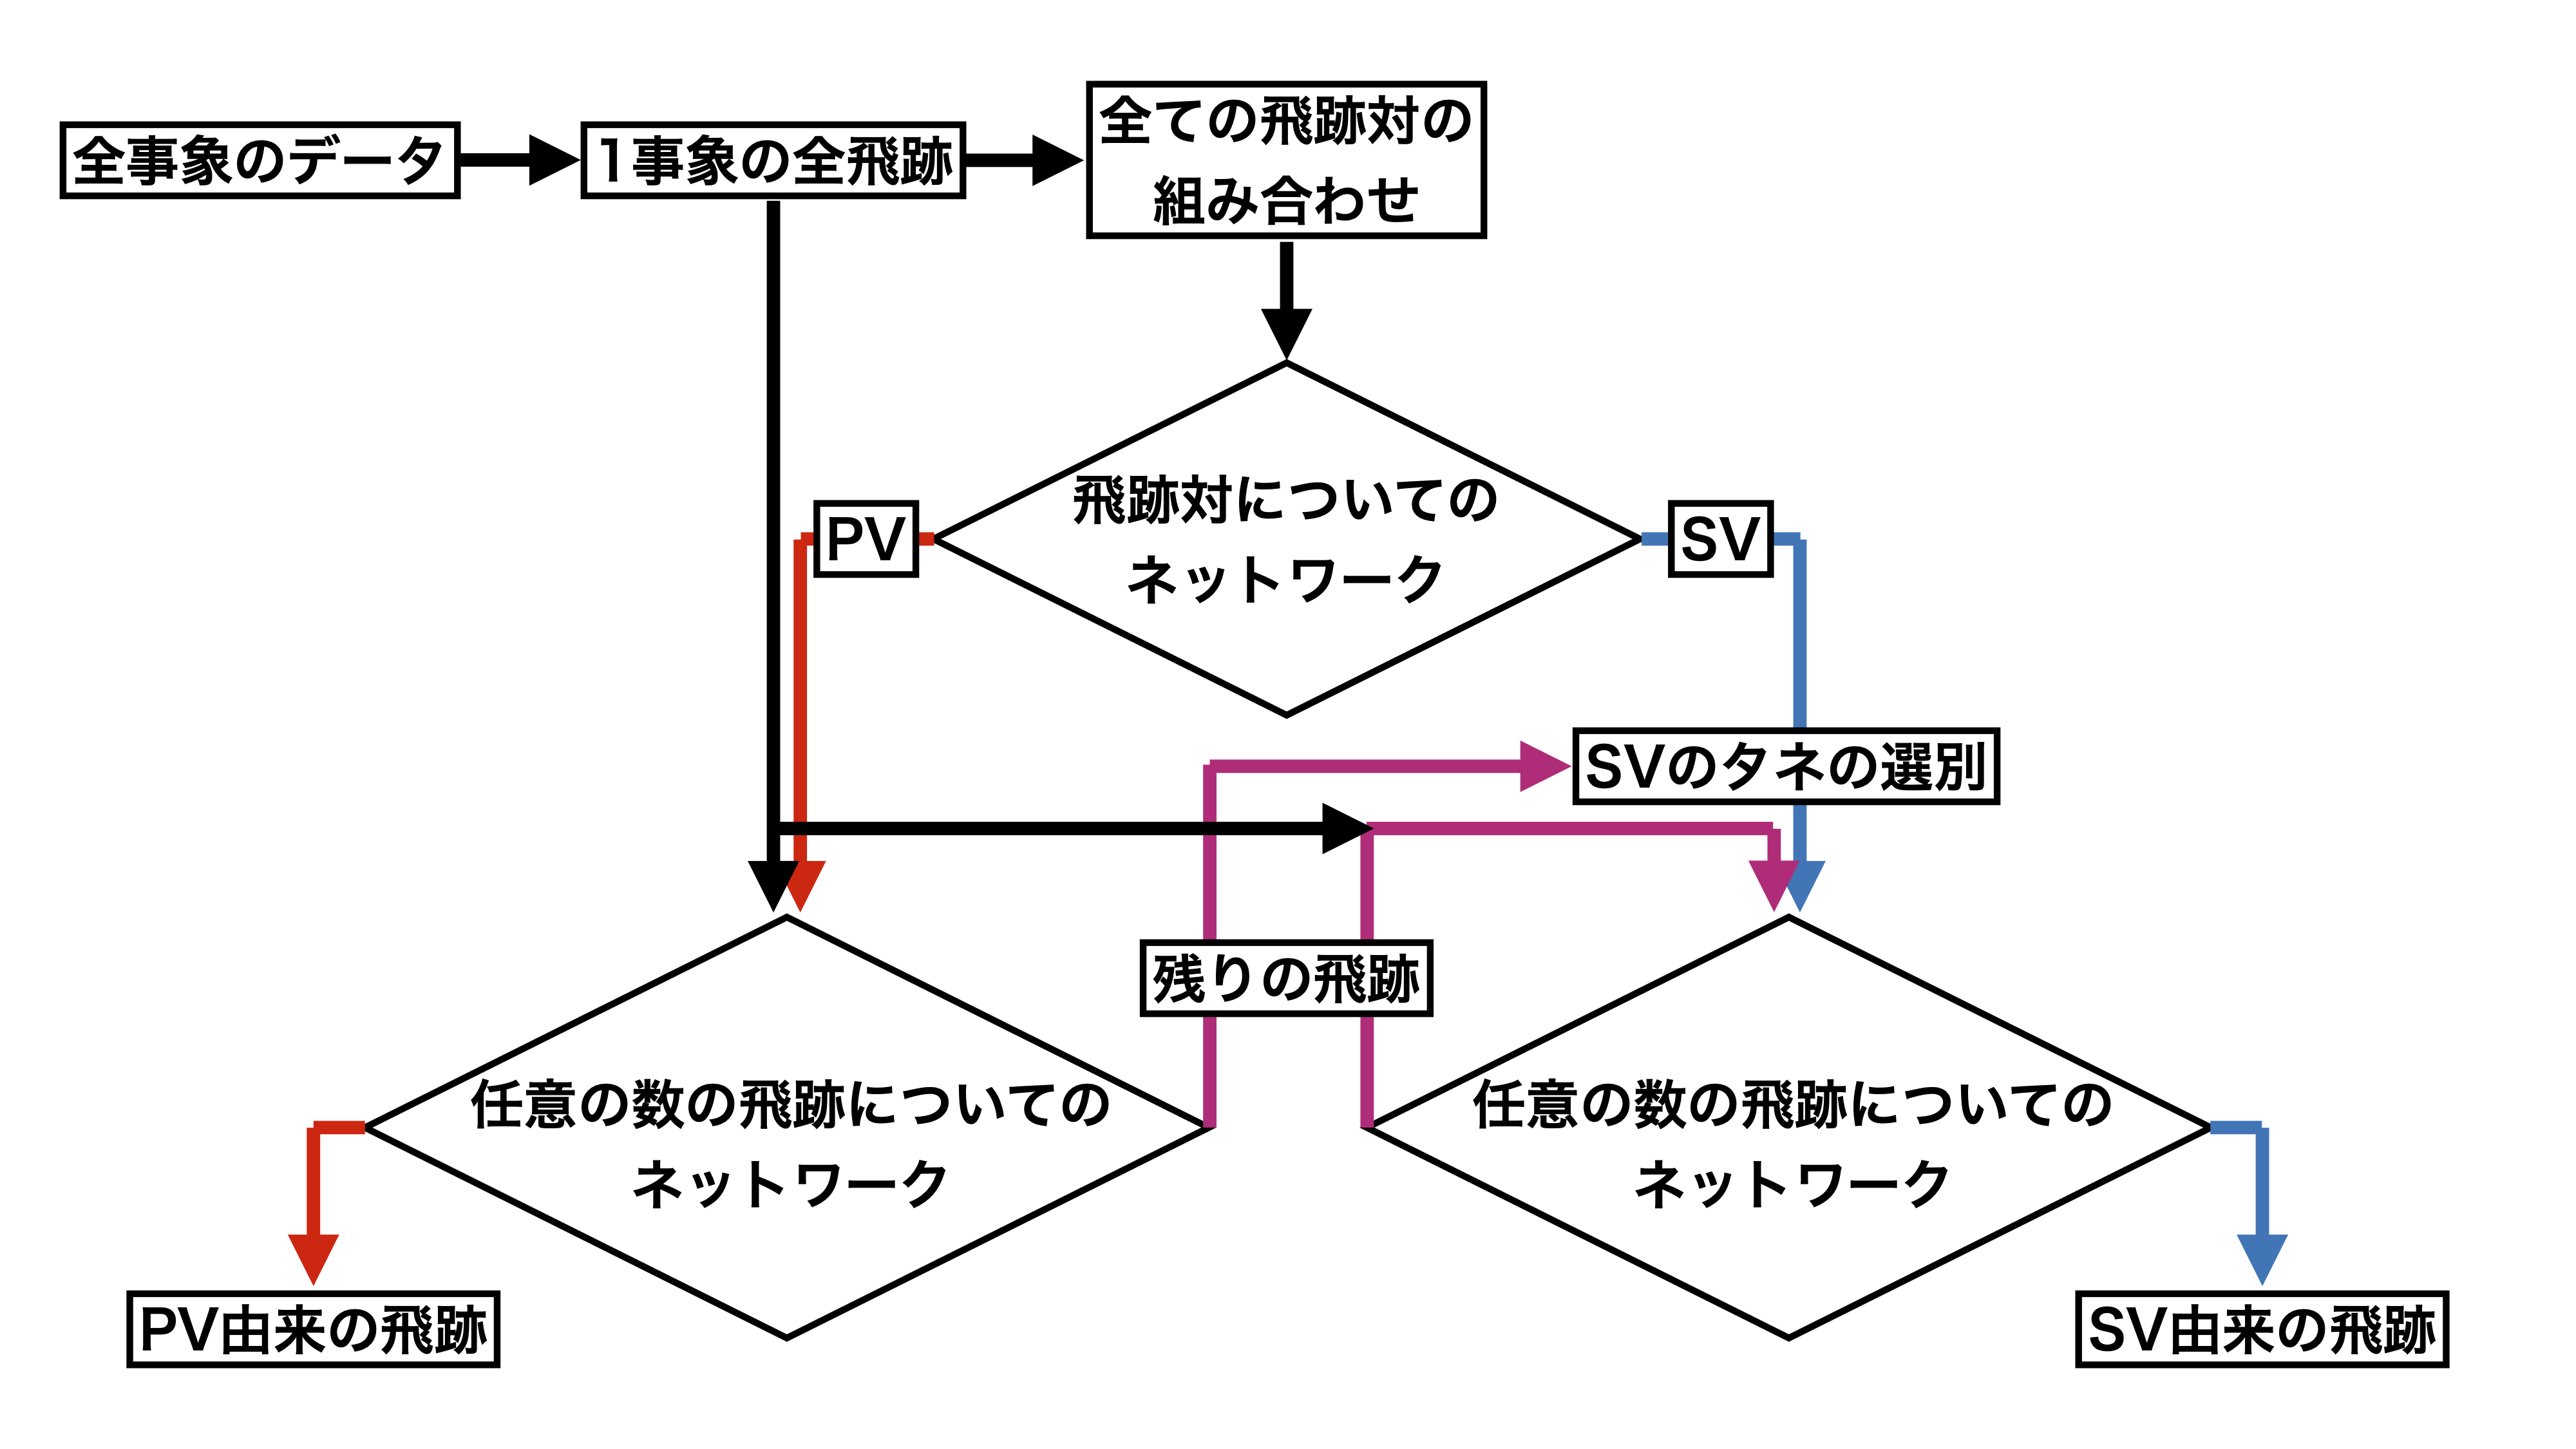
\includegraphics[width=0.9\textwidth, clip]{Figure/4VertexFinderwithDL/4-1-0-1VertexFinderAlgorithm.png}
 \caption{崩壊点検出アルゴリズム}
 \label{4-1-0-1VertexFinderAlgorithm}
\end{figure}

アルゴリズムは以下の手順で崩壊点の再構成を行う。

\begin{enumerate}
 \item 全事象から1事象分のデータを取り出し、全ての飛跡対の組み合わせを考える。
 \item それら飛跡対に対して、飛跡対についてのネットワークを使用し、崩壊点のタネの探索を行う。
 \item SVと判定された飛跡対について、選別を行いSVのタネを選ぶ。
 \item PVと判定されたタネについて、任意の数の飛跡についてのネットワークを用いPVの生成を行う。
 \item SVのタネとPV由来の飛跡の情報を用い、任意の数の飛跡についてのネットワークによってSVのタネが無くなるまでSVを生成する。
\end{enumerate}

手順1、2については飛跡対についてのネットワークの訓練データの作成や学習と全く同様の手順である。

手順3では、飛跡対についてのネットワークによって得られるSVCC・SVBB・TVCC・SVBCのスコアや崩壊点の位置を用いてより純度の高いSVのタネの集合を作成する。
したがって、SVCC・SVBB・TVCC・SVBCのスコアについての閾値や崩壊点の位置についての最適化が必要である。

手順4では、飛跡対についてのネットワークによって得られるPVのスコアに関して降順に並び替えたPVのタネに対して、個々に任意の数の飛跡についてのネットワークを用いPVを生成する。
ここでは、幾つのPVのタネを用いるかの最適化が必要である。
また一度以上、任意の数の飛跡についてのネットワークによって結合していると判定された飛跡をPV由来であると判断している。
この時の任意の数の飛跡についてのネットワークによって得られるスコアについての閾値についてもまた同様に最適化が必要なパラメータである。

手順5について、手順3で選別したSVのタネと手順4で得られたPV由来であると判定された飛跡の一覧を用いてSVの再構成を行う。
ここでは任意の数の飛跡についてのネットワークのデコーダー部に入力する飛跡から、再構成されたSV由来の飛跡を取り除いて行くことによって、再帰的にSVの生成が行われる。
SVのタネに含まれる飛跡はPV由来の飛跡の一覧になく、かつそれまでに生成したSV由来の飛跡の一覧にもないものを用いる。
このSVに関する任意の数の飛跡についてのネットワークのスコアも最適化が必要である。
また、再構成されたSV由来の飛跡の一覧にPV由来の飛跡が存在した場合は任意の数の飛跡についてのネットワークによって得られたスコアによって飛跡の争奪が行われる。
手順5はSVのタネが無くなるまで行われ、再構成されたSV由来の飛跡とPV由来の飛跡以外の飛跡は残りの飛跡とする。

以上が崩壊点検出のためのアルゴリズムである。
最適化が必要なパラメータを以下にまとめる。

\begin{itemize}
 \item 飛跡対についてのネットワークによって得られるSVCC・SVBB・TVCC・SVBCのスコアについての閾値
 \item 飛跡対についてのネットワークによって得られる崩壊点の位置についての閾値
 \item 使用するPVのタネの数
 \item PVの生成に関する任意の数の飛跡についてのネットワークによって得られるスコアについての閾値
 \item SVの生成に関する任意の数の飛跡についてのネットワークによって得られるスコアについての閾値
\end{itemize}

%%%%%%%%%%%%%%%%%%%%%%%%%%%%%%%%%%%%%%%%%%%%%%%%%%%%%%%%%%%%%%%%%%%%%%%%%%%%%%%%%%%%%%%%%%%%%%%%%%%%%
\section{崩壊点検出の最適化と評価} \label{VFDL:TuneandPerformanceofVFDL}

崩壊点検出に関しての性能を以下の基準で評価する。

評価項目とか。\\
飛跡レベルでの効率。\\

%%%%%%%%%%%%%%%%%%%%%%%%%%%%%%%%%%%%%%%%%%%%%%%%%%%%%%%%%%%%%%%%%%%%%%%%
\subsection{Primary Vertexの再構成} \label{VFDL:AlgoVFDL:ReconstructionofPrimaryVertex}

\ref{Net:PM:PerformanceofPM}項で示したように飛跡対のクラスはNCが支配的なデータとなっており、分類問題の結果においてもNCからの汚染が顕著であった。
これは図\ref{3-1-1-2TracksandVertices}からも分かるようにPV由来の飛跡が比較的多く、これらPV由来の飛跡とそれぞれのSV由来の飛跡によって構成される飛跡対が非常に多くなるためである。
したがって、このNCに分類される飛跡対はPV由来の飛跡を精度よく見分けることができれば大幅に減らすことが可能であると考えられる。

ここではそのようなPVの再構成について評価を行う。
ただし、アルゴリズムでも述べたようにPV由来の飛跡はその任意の数の飛跡についてのネットワークから得られるスコアによってはSVに分類される為、最終的な結果はここで得られる効率や純度とは異なっている。
PVの再構成は、飛跡対についてのネットワークによって得られたPVのタネと事象中の全ての飛跡を用いて行われる。
まず、PVのタネは飛跡対についてのネットワークにおけるスコアによって降順にソートされ、スコアの高いタネから順に使用される。
この時、PVのタネを幾つ使用するかという値を、ループ数と呼ぶと事する。
PVのタネは任意の数の飛跡についてのネットワークに入力され、それぞれのタネについてPVが生成される。
ここでは少なくとも一度PVと任意の数の飛跡についてのネットワークによって判定された飛跡をPV由来の飛跡して数えることとする。
ループ数は多ければ多い程、PVに関しての効率が上がり、純度が下がる変数である。
また、飛跡対についてのネットワークが誤ったタネを提供してしまう可能性があることを考慮しなければならない。
横軸にループ数、縦軸にタネの正答率をとったグラフを図\ref{}に、同様に縦軸にPVに関しての効率と純度をとったグラフを図\ref{}に示す。

ここでPVに関しての効率を"MCによってPVとラベルされた飛跡の内、ネットワークがPVと選択できた飛跡の割合"、純度を"ネットワークがPVと選択した飛跡の内、MCによってPVとラベルされた飛跡の割合"と定義した。

一方、任意の数の飛跡についてのネットワークから得られる各飛跡についてのスコアに対しても閾値を設けなければならない。
図\ref{}や図\ref{}ではこの閾値を$0.5$としていた。
これは二値分類における標準的な閾値である。
それぞれのループ数に対して、横軸に任意の数の飛跡についてのネットワークに関するスコアの閾値、縦軸に効率と純度をとったグラフを図\ref{}に示す。


PVの再構成では後述するSVのタネの純度を高くする為、効率を重視している。
したがって、これらのパラメータの値として、ループ数を$3$、スコアの閾値を$0.5$とする。


%%%%%%%%%%%%%%%%%%%%%%%%%%%%%%%%%%%%%%%%%%%%%%%%%%%%%%%%%%%%%%%%%%%%%%%%
\subsection{Secondary Vertexのタネの選別} \label{VFDL:AlgoVFDL:SelectionofSecondaryVertexSeed}

SVのタネに関しては、その純度をより向上させる為、タネの選別を行なっている。
SVのタネは以下の基準で選択される。

\begin{enumerate}
 \item PV由来の飛跡に含まれていない。
 \item 崩壊点のタネがSVCC・SVBB・TVCC・SVBCのいずれかである。
 \item SVCC・SVBB・TVCC・SVBCのスコアの和が閾値以上である。
 \item 崩壊点の位置が閾値以下である。
\end{enumerate}

以上の基準について、SVCC・SVBB・TVCC・SVBCのスコアの和についての閾値や、崩壊点の位置についての閾値に関しては調整が必要なパラメータである。
横軸をSVCC・SVBB・TVCC・SVBCのスコアの和についての閾値、縦軸を崩壊点の位置の閾値、カラースケールをタネの正答率としたグラフを図\ref{}に示す。

ここで、MCによってSVBCとラベル付された飛跡対に関しては崩壊点のタネから除外している。
また、基準1、基準2によって除外されたSVのタネについても除外している。

実際にはSVのタネは更にSVの生成によって取り除かれた飛跡を考慮し、常に飛跡対の両方が飛跡のリストに入っていることを要求している。




\section{崩壊点検出の性能} \label{VFDL:SummaryofVFDL}






















